\section{System Architecture}

The architecture of the system we proposed can be seen at
\ref{system-architecture}.
We can separate the deployment into 4 groups.
\begin{enumerate}
    \item The first one, the ESP32, are the physical device
          that gathers the air quality data and controls the door.
    \item Second, the Application Server are the primary brain
          of the whole system from collecting the data
          retrieved from the ESP32, saving the data, to
          managing the state of the system.
    \item Third, the SparkMachine, are the processor of data
          that processes the data into more meaningful
          informations for the user, such as minimum, maximum,
          and average values.
    \item Lastly, the User Device are users' devices that
          accesses the web application to interact with the
          system.
\end{enumerate}

\begin{figure}
    \centerline{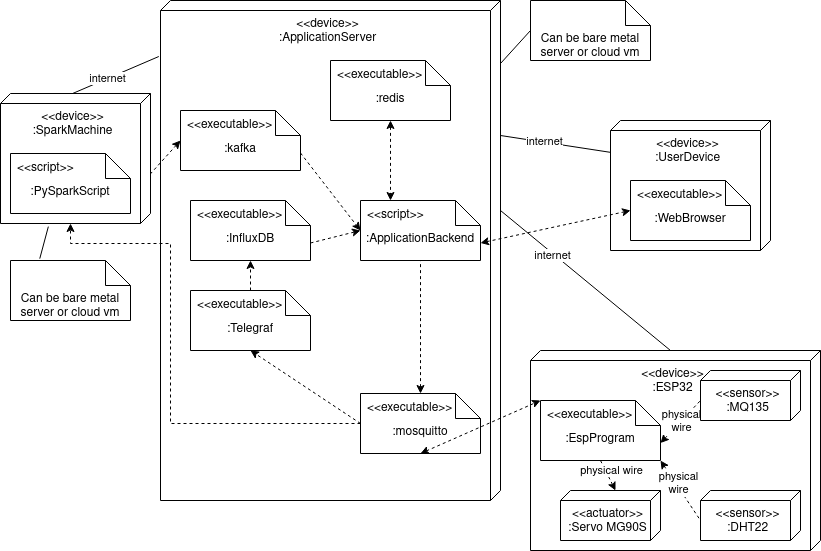
\includegraphics[scale=0.3]{resources/deployment-diagram.png}}
    \caption{Deployment diagram of the smart room air conditioner}
    \label{system-architecture}
\end{figure}

Flow-wise, the data gathered by the MQ135 and DHT22, in the
ESP32, are sent to the mosquitto, the MQTT broker, in the
Application Server.
There, the data are consumed by both Telegraf in the
Application Server to be saved into the InfluxDB, and
PySparkScript in the SparkMachine to be processed into
minimum, maximum, average, and median values.

The sensor data in InfluxDB and the processed data are then
used to be displayed as a statistic of the web application.
The sensor data are also used as training data for the KMeans
algorithm to determine the air quality level of each
indicators. The current average of each indicators are then
passed to the KMeans model to determine the current air
quality level of the room, thus determining whether the door
should be opened or closed.
